\subsection{Evaluation of objects lists - Post-processing}
To evaluate the quality of calculated sensor data with the aim to improve the object detection algorithm post-processing is necessary.
After recording objects lists data streams in Rosbag files there is the possibility to analyze data in different ways by multiple post-processing functions. 
Either a single Rosbag file can be analyzed or two files can be compared. In both cases the data is evaluated frame by frame. 

\subsubsection{Basic analysis}

Considered to one single Rosbag file specific attribute values of single objects which are selected by their object \ac{ID} can be displayed. The variety of available attribute types is described in \cref{B}. In addition, the number of detected objects can be visualized. \\

\subsubsection{Advanced analysis}
\label{sssec:eval}

Regarding two Rosbag recordings further analysis methods for comparing the streams are provided. In this case a common time base needs to be generated. To avoid errors because of time variation of both recordings following mapping algorithm is executed. Each frame time stamp is handled as time relative to its Rosbag start time in milliseconds. To every frame in the Rosbag file which is provided by sensor data a frame of simulation data is dedicated. The simulation frame to choose is the latest past frame in relative stream time. The principle of frame mapping is shown in figure \ref{fig:frame_mapping}. With this mechanism pairs of frames are generated (sensor frame with corresponding simulation frame).

\begin{figure}[t]
	\centering
	\fbox{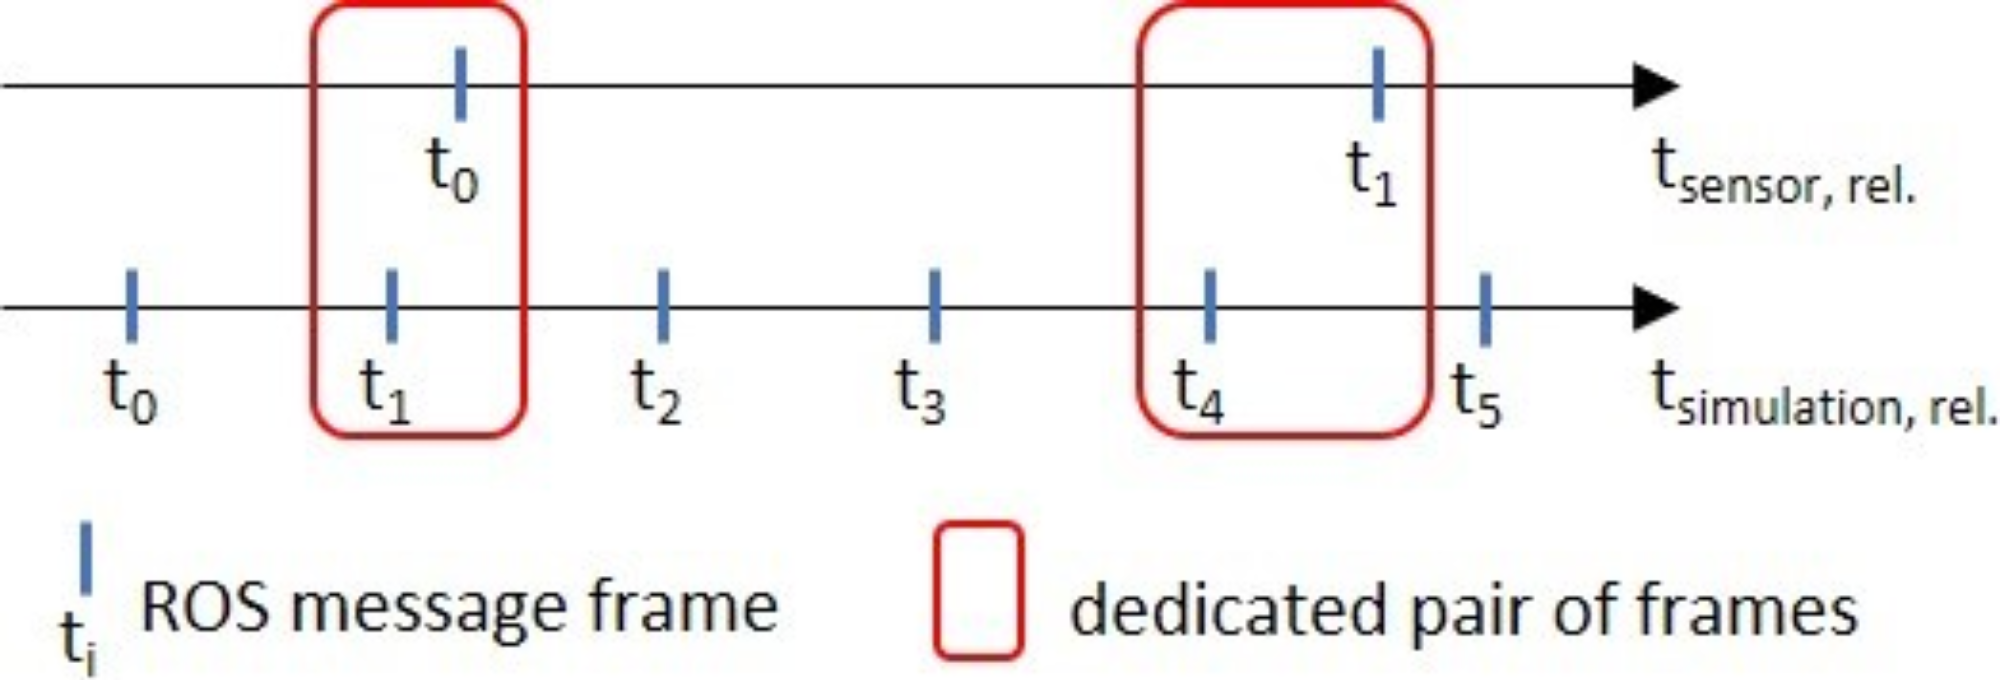
\includegraphics[width=\linewidth]{canvas}}
	\caption{Principle of frame mapping algorithm}
	\label{fig:frame_mapping}
\end{figure}

A fundamental use case in analysing the recorded Rosbag files is to evaluate the quality of sensor data in comparison with GT data through metrics introduced in \cite{Reway}. 
To determine whether a given camera object is evaluated as \ac{TP}, \ac{FP}, \ac{FN} or a \ac{mm}, the \textbf{\ac{IoU}} value is used. 
In general there is a list of $m$ camera objects ($B_{pr}$) and a list of $n$ \ac{GT} objects ($B_{gt}$) for each frame. To evaluate a frame, for each combination of GT object and camera object the IoU value is calculated. All those values build a matrix like shown in \cref{tab:matrix}.
\begin{table}[h]
	\caption{IoU-Matrix for a single frame}
	\begin{tabularx}{\columnwidth}{X|X|c|X}
		\toprule
		$IoU(B_{gt,1}, B_{pr,1})$ & $IoU(B_{gt,2}, B_{pr,1})$ & ... & $IoU(B_{gt,n}, B_{pr,1})$ \\
		\midrule
		$IoU(B_{gt,1}, B_{pr,2})$ & $IoU(B_{gt,2}, B_{pr,2})$ & ... & $IoU(B_{gt,n}, B_{pr,2})$ \\
		\midrule
		... & ... & ... & ... \\
		\midrule		
		$IoU(B_{gt,1}, B_{pr,m})$ & $IoU(B_{gt,2}, B_{pr,m})$ & ... & $IoU(B_{gt,n}, B_{pr,m})$ \\
		\bottomrule
	\end{tabularx}
	\label{tab:matrix}
\end{table}

After calculating the matrix the objects in one single frame can be evaluated. A given camera object $B_{pr,i}$ is ... \\

... \textbf{FP} if there is no value 
\begin{equation}
	IoU(B_{gt,k}, B_{pr,i}) > t \text{\quad with\quad} k \in \left\lbrace 1, ..., n\right\rbrace 
	\label{eq:fp_case}
\end{equation}
in the according row of the matrix which is greater than the given threshold $t$. \\

... \textbf{FP} if there is one or more IoU values in the according row greater than the threshold, but for every $B_{gt,k}$, for which expression \cref{eq:fp_case} is true, there is another $B_{pr,j}$ ($j\neq i$) which matches with $B_{gt,k}$ and $IoU(B_{gt,k}, B_{pr,j}) > IoU(B_{gt,k}, B_{pr,i})$ \\

... a \textbf{\acf{mm}} if it is no FP case, but none of the found possible matching $B_{gt,k}$ has the same class as $B_{pr,i}$. \\

... \textbf{TP}, also called a match, if none of the other mentioned cases are detected. That means, that there is at least one $B_{gt,k}$ which fulfills expression \cref{eq:fp_case} and has the same classification as $B_{pr,i}$ and there is no other $B_{pr,j}$ which matches better with the found $B_{gt,k}$. \\

Going through the rows of the matrix, for each $B_{pr,i}$ in the given frame it can be decided, whether the case is TP, FP or mm. \\

The other way round, examining the \ac{GT} objects $B_{gt,k}$, that means the columns of the calculated matrix, all FN cases can be detected. It is an \textbf{FN} if there is no $B_{pr,i}$ for which
\begin{equation}
	IoU(B_{gt,k}, B_{pr,i}) > t \text{\quad with\quad} i \in \left\lbrace 1, ..., m\right\rbrace 
	\label{eq:fn_case}
\end{equation}
Going through the columns of the matrix, this decision can be made for every $B_{gt,k}$. \\
With these steps, a given frame with $m$ camera objects and $n$ \ac{GT} objects can be investigated. \\

These functions, one for investigating the camera objects and one for detecting all FN cases, were realized in Python. The calculation of an IoU value is processed with functions of the package \textit{shapely} \cite{Shapely}.
First, the given objects which are defined through their properties \textit{x}, \textit{y}, \textit{length}, \textit{height}, \textit{yaw} and \textit{classification} like presented in \cite{Aeberhard}
are transformed into bounding boxes. With two of these bounding boxes \textit{shapely} can calculate the intersection area and the union area so that the IoU value can be processed. \\

As a result of the frame evaluation functions following data quality parameters according to \cite{Reway} can be calculated:
\begin{itemize}
	
	\item recall per frame
	\item precision per frame
	\item FPPI per sensor data stream 
	\item MOTA per sensor data stream 
	\item MOTP per sensor data stream 
	
\end{itemize}

Another feature of the post-processing application is the analysis of deviations by calculating differences of specific attribute values between two recorded data streams. For that matter only \ac{TP} cases of IoU evaluation are regarded and the concerning object is selected by its object \ac{ID} in the simulation data record. The difference value results from
\begin{equation}
	difference = value_{simulation} - value_{sensor} 
	\label{eq:diff}
\end{equation}

\subsubsection{\ac{GUI}}
To investigate the quality of the processed camera object data, a \ac{GUI} is provided. It is designed with Python's binding package for Qt (PyQt5) \cite{PyQt5} and defined as a plugin for \textit{rqt}, a \ac{ROS} framework for \ac{GUI} development \cite{rqt}.
With this plugin, the user can import two Rosbag files, one GT data file and one sensor (camera) data file.
By using the functions mentioned before, the \ac{GUI} can show several data graphs to the user like raw data plots, comparing plots with object data of both files or evaluation data. 
Along with every data set - except from FPPI, MOTA and MOTP - the mean value and the standard deviation for each data set is portrayed in the \ac{GUI}. \\
Apart from data plots the interface can also show quality parameters for the whole camera data Rosbag file in an extra widget. For each operation where IoU calculation is needed, the user can set the threshold value for the evaluation. 